%\begin{figure*}[!t]
%	\begin{center}
%		\subfigure[No Failure]
%		{
%			\label{fig:sc_no_fail}
%			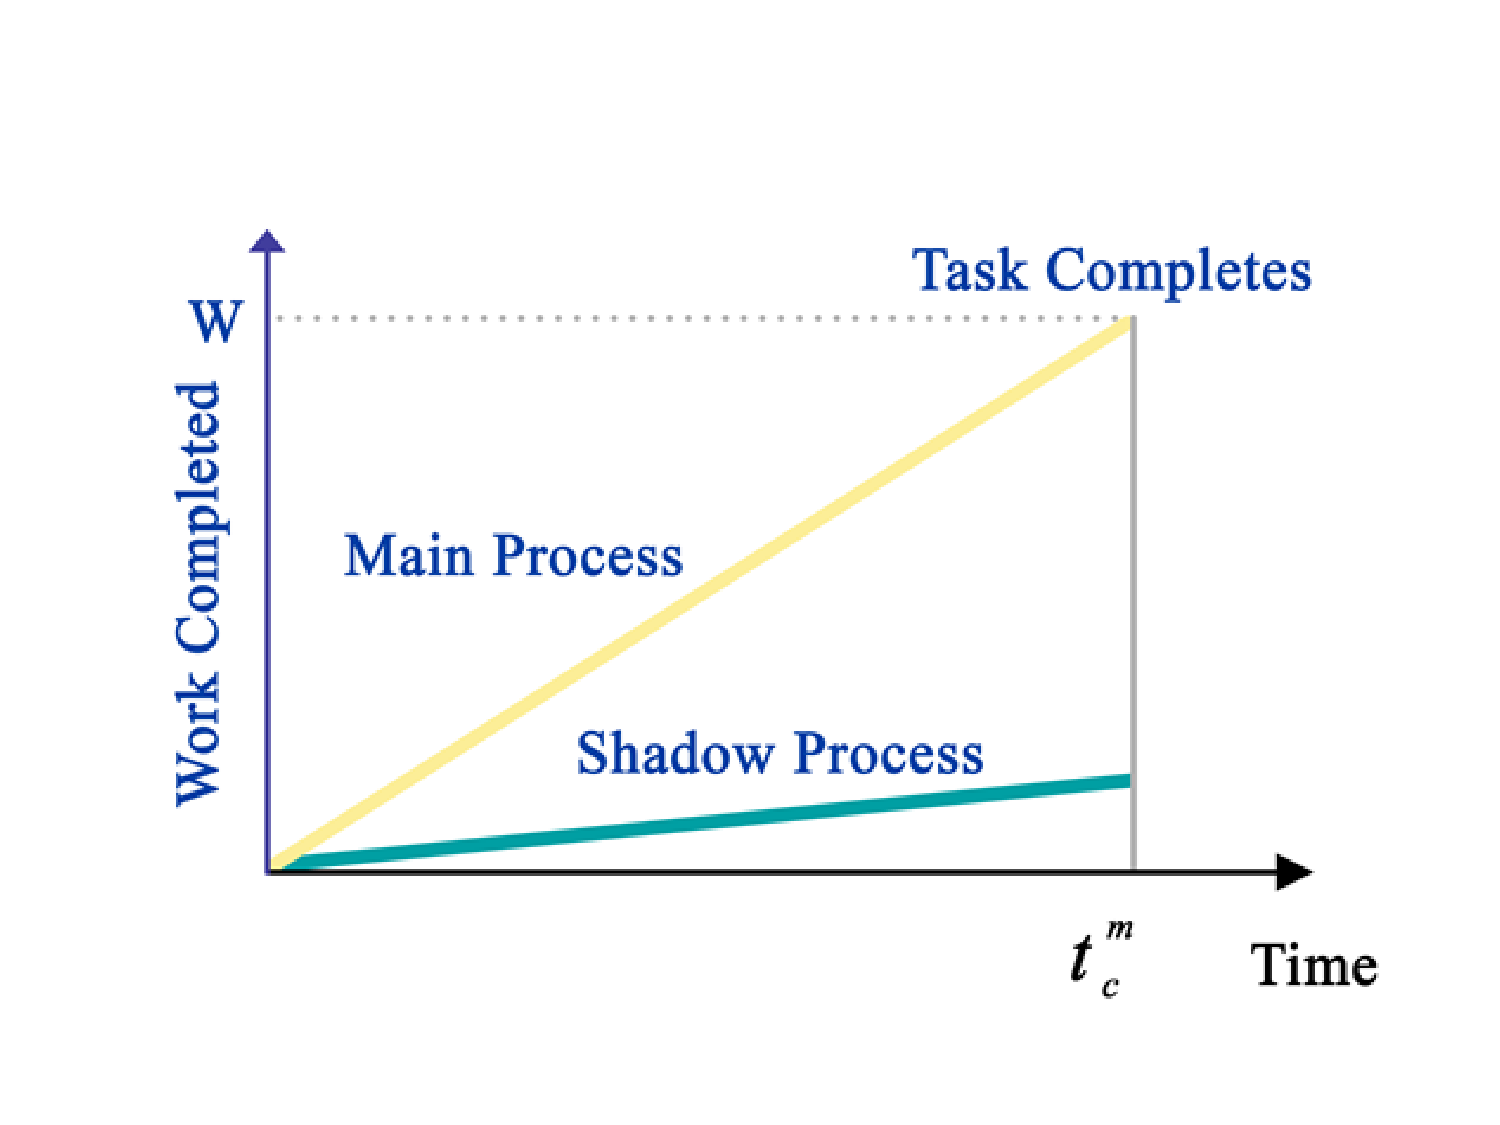
\includegraphics[width=0.32\textwidth]{Figures/example1.pdf}
%		}
%		\subfigure[Shadow Process Failure]
%		{
%			\label{fig:sc_shadow_fail}
%			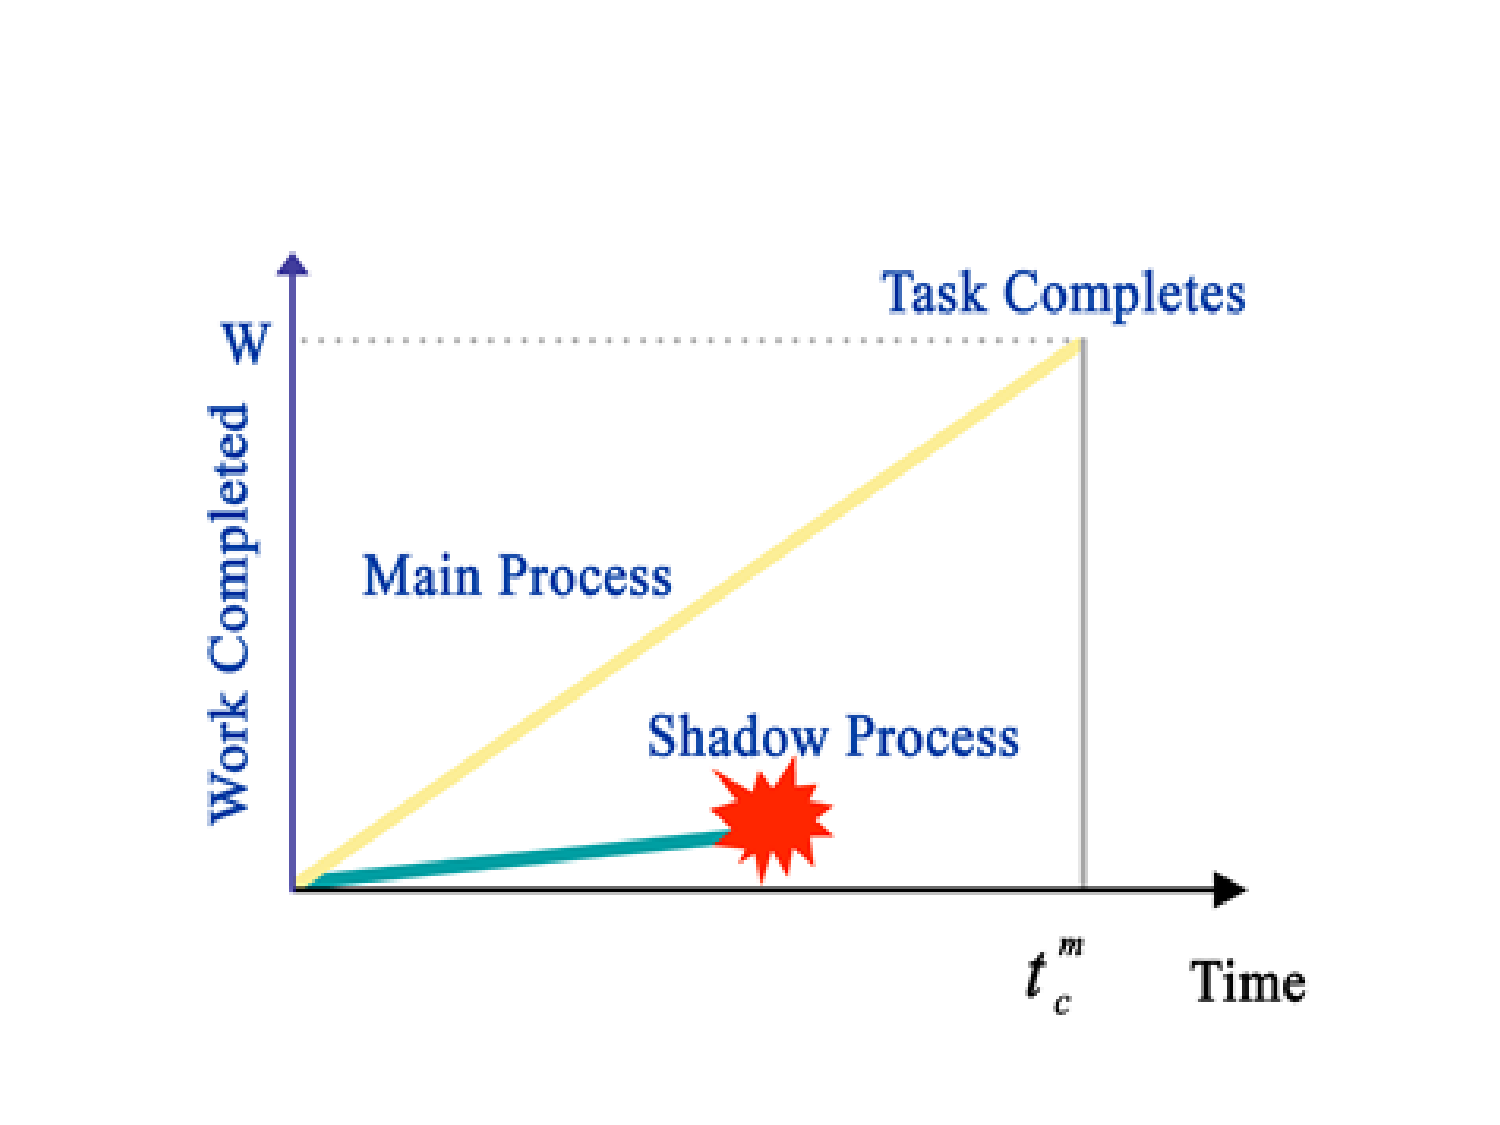
\includegraphics[width=0.29\textwidth]{Figures/example3.pdf}
%		}
%		\subfigure[Main Process Failure]
%		{
%			\label{fig:sc_main_fail}
%			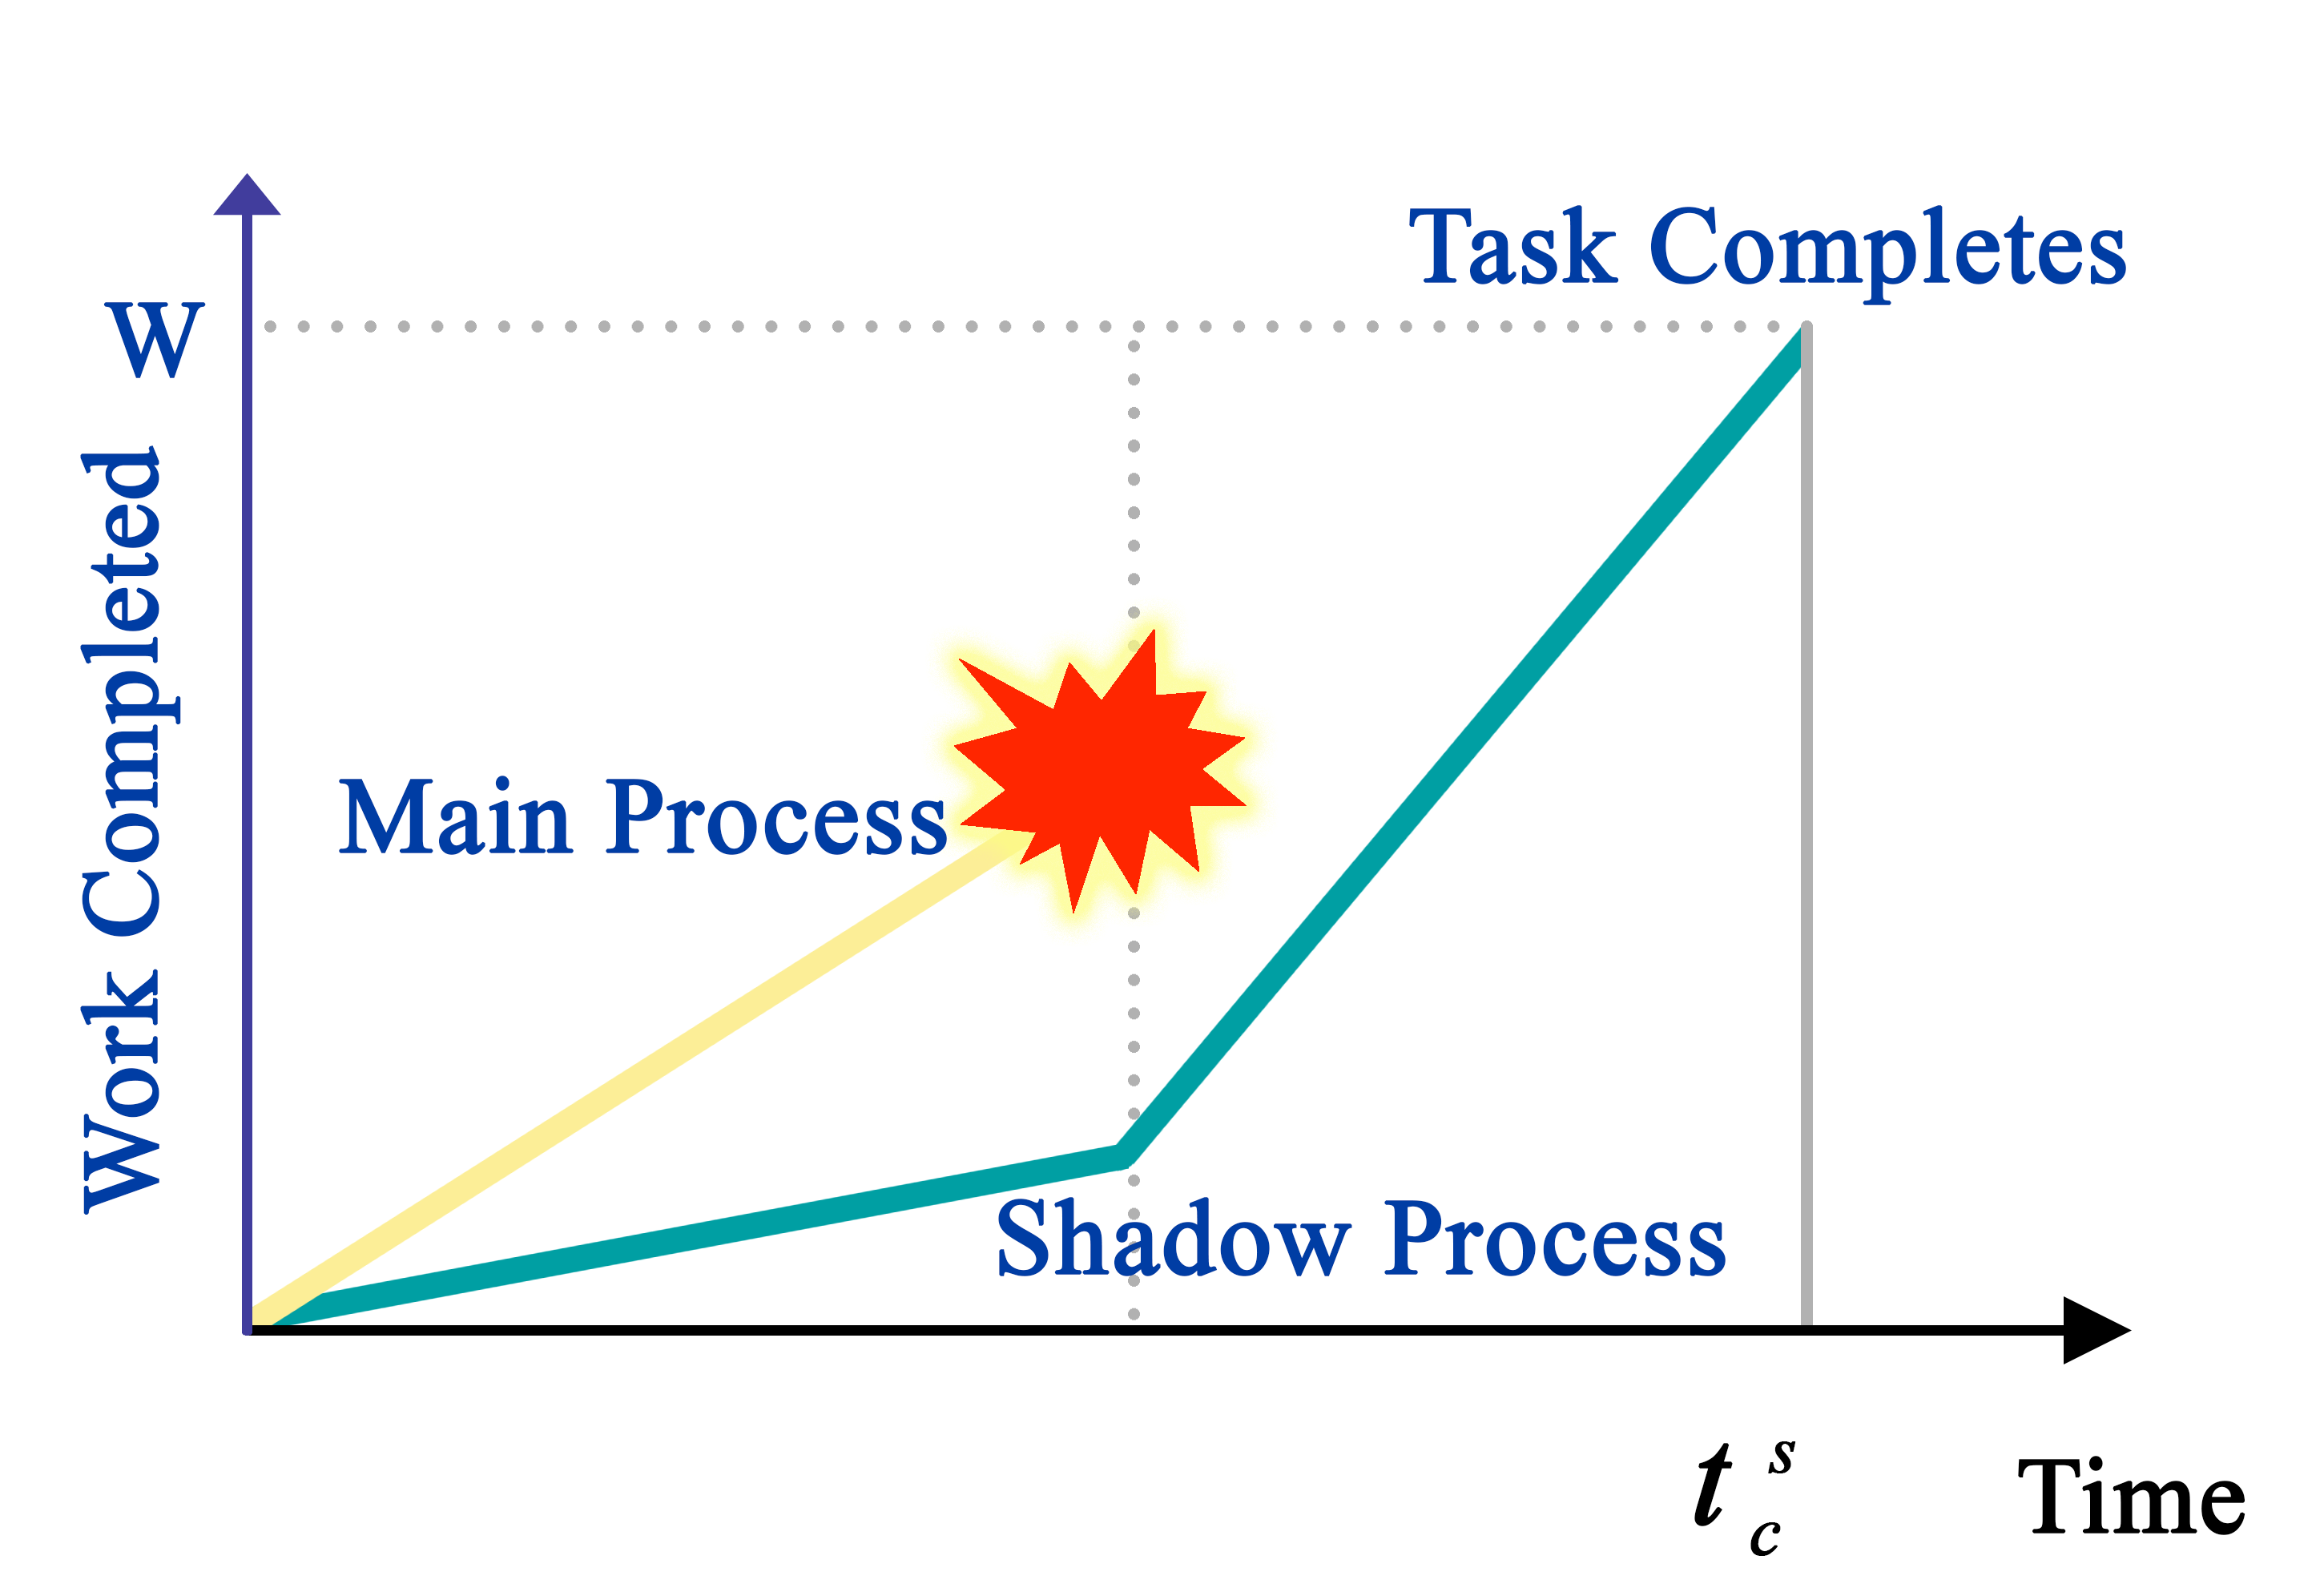
\includegraphics[width=0.33\textwidth]{Figures/example2.png}
%		}
%	\end{center}
%	\caption{Shadow Replication with a single shadow process.}
%	\label{fig:sc_overview}
%	\end{figure*}

The basic tenet of the proposed fault tolerance framework, referred to as Leaping Shadows, is the concept of shadowing, whereby each main process is guarded by a suite of ``shadow" processes. To finish a task, the shadow processes will execute the same code as its associated main process, and the task will be successfully completed as long as one of the processes can finish. %, whose size depends on the criticality of the application and hardware and power budget. 
%To mitigate correlated failures, the main and shadow processes
%execute on separate computing nodes.
The novelty of Leaping Shadows lies in its dynamic and differential adjustment of the execution rates. Specifically, it 
executes the main processes at the rate required for response time constraint, while slowing down the shadows to reduce hardware and 
power requirement. Upon failure of a main process, 
its associated shadow increases its rate to complete the task, thereby reducing the delay to the progress of other tasks. 
 
Leaping Shadows is adaptive in four dimensions. Firstly, the number of shadow processes to use for each main process can be decided  
to balance the trade-off between the criticality of the application, and hardware and power budget. Secondly, the execution rates of the main and shadow processes are tunable performance determinants. Thirdly, if compute nodes exhibit different ``health" status, partial shadowing, where only processes running on ``weak" nodes are shadowed, can be applied to minimize resource usage. Last but not least, instead of slowing down, the shadows may execute reduced code, e.g. with less resolution, to generate less precise results in the case of failure.

 %, thereby enabling a parameterized trade-off between response time and energy consumption.


%Leaping Shadows is a generalization of existing fault tolerance
%approaches. %, namely Checkpoint/restart and Process Replication. 
%Specifically, if there is enough laxity in response time constraint, Shadow
%Computing would start the shadows only after the main instance fails, mimicking Re-execution. %It is clear, therefore, that for a
%large response time, Shadow Replication converges to re-execution, as
%the shadow remains idle during the execution of the main process and
%only starts execution upon failure. 
%If the target response time is
%stringent, however, %Shadow Replication converges to process replication,
%the shadows would execute simultaneously with the main at the maximal
%rate, mimicking Process Replication. The flexibility of Shadow Replication provides a spectrum
%of fault tolerance strategies that strike a
%balance between completion time and energy saving.


\subsection{Execution rate control}
\vspace*{-2mm}
One challenge in Leaping Shadows is how to control the execution rates. So far, we have explored two methods to differentiate the execution rates. The first approach is to use Dynamic Voltage and Frequency Scaling (DVFS), of which the CPU frequency scales linearly with the supply voltage~\cite{cui_en7085151,cui_closer_2014}. The second approach is to use time sharing to reduce the effective execution rate while keeping the compute nodes running at maximal frequency. Since this approach collocates multiple processes  on a same node, it simultaneously reduces the number of machines to be used and the power consumption~\cite{cui_ics_2015}.

\subsection{Modeling and Simulation}
\vspace*{-2mm}
The other challenge resides in determining
jointly the execution rates of all processes, %both before and
%after a failure occurs, 
with the objective to minimize power consumption while satisfying QoS requirements. To achieve this, I propose two analytical
models, corresponding to the two rate-control approaches above. The models consider the time and power needed for a job, %which is composed of multiple parallel tasks, 
under different system specifics and failure distributions. From the analytical models an optimization problem is formulated and solved to derive the optimal execution rates.  %The profit is modeled as the difference between the payment from customers, which depends on the completion time, and expenses for running the cloud job, which are mainly energy costs. %Afterwards, an optimization problem is formulated to derive the optimal execution rates. 
%For more details please refer to~\cite{cui_en7085151}. 

To verify the correctness of the analytical models, I build an event-driven simulator that simulates the behaviors of Leaping Shadows under different system specifics, task characteristics, and failure distributions. It can report all necessary statistics, such as number of failures encountered, time to completion, and energy consumption. The statistics can then be used to compare with the results from the analytical model.

\subsection{Implementation}
\vspace*{-2mm}
I am actively implementing Leaping Shadows as a runtime for Message Passing Interface (MPI), which is the de facto programming paradigm for HPC. 
Instead of a full-feature MPI implementation, the runtime is designed to be a separate layer between MPI and user application, in order to take advantage of existing MPI performance optimizations that numerous researches have spent years on. 
The runtime spawns the shadow processes, manages the coordination between main and shadow processes, and guarantees consistency for messages and non-deterministic events. 

\subsection{Results}
\vspace*{-2mm}
Several important factors are identified that impact the performance of Leaping Shadows. Correspondingly, I conduct a series of sensitivity studies where Leaping Shadows is compared to state-of-the-art approaches. %The influential parameters can be classified into three categories, i.e., system specifics, SLA specifics, and job specifics. Further, the system specifics includes static power/dynamic power ratio and failure distribution, the job specifics includes workload and number of tasks, and SLA specifics is mainly targeted job completion time 
The results from both the analytical model and simulator show that Leaping Shadows can achieve significant power/energy savings, without violating the QoS constraints. %Specifically, I conducted 4  sensitivity studies. 
%Specifically, Leaping Shadows can achieve 15\%-30\% energy savings under normal configurations. Furthermore, Leaping Shadows would converge to Process Replication, when target response time is stringent, and to Re-execution when target response time is relaxed or when failure is unlikely.%~\cite{cui_closer_2014}.




